%%%%%%%%%%%%%%%%%%%%%%%%%%%%%%%%%%%%%%%%%%%%%%%%%%%%%%%%%%%%%%%%%%%%%%%%%%%%%%%%%%%
%% This project aims to create the template for presentation.                   %%
%% author: Luigi Durso                                                          %%
%% contacts:                                                                    %%
%%    e-mail: luigi.durso@si2001.it                                             %%
%%    linktree: https://linktr.ee/maumneto                                      %%
%%%%%%%%%%%%%%%%%%%%%%%%%%%%%%%%%%%%%%%%%%%%%%%%%%%%%%%%%%%%%%%%%%%%%%%%%%%%%%%%%%%
\documentclass{../libs/presentation_format}
% Inserting the preamble file with the packages
%%%%%%%%%%%%%%%%%%%%%%%%%%%%%%%%%%%%%%%%%%%%%%%%%%%%%%%%%%%%%%%%%%%%%
%% This file contains the packages that can be used in the beamer. %%
%%%%%%%%%%%%%%%%%%%%%%%%%%%%%%%%%%%%%%%%%%%%%%%%%%%%%%%%%%%%%%%%%%%%%
% Package to fonts family
\usepackage[T1]{fontenc}
% Package to accentuation
\usepackage[utf8]{inputenc}
% Package to Italian language
\usepackage[italian]{babel}
% Package to Figures
\usepackage{graphicx}
\usepackage{caption}
\usepackage{subcaption}
% Package to the colors
\usepackage{color}
% Package to the colors
\usepackage{xcolor}
% Packages to math symbols and expressions
\usepackage{amsfonts, amssymb, amsmath}
% Package to multiple lines and columns in table
\usepackage{multirow, array} 
% Package to create pseudo-code
% For more detail of this package: http://linorg.usp.br/CTAN/macros/latex/contrib/algorithm2e/doc/algorithm2e.pdf
\usepackage{algorithm2e}
% Package to insert code
\usepackage{listings} 
\usepackage{keyval}
% Package to justify text
\usepackage[document]{ragged2e}
% Package to manage the bibliography
\usepackage[backend=biber, style=numeric, sorting=none]{biblatex}
% Package to facilities quotations
\usepackage{csquotes}
% Package to use multicols
\usepackage{multicol}
% Inserting the references file
\bibliography{../references.bib}

% Title
\title[Flutter-Dart]{\huge\textbf{Flutter e Dart - Le basi}}
% Subtitle
\subtitle{Flutter - Applicazioni multipagina}
% Author of the presentation
\author{Luigi Durso}
% Company's Name
\institute[SI2001]{
    % email for contact
    \normalsize{\email{luigi.durso@si2001.it}}
    \newline
    \centering
    
\includegraphics[scale=0.3]{../libs/emblem.png}
    \newline
    % company name
    \company
}
% date of the presentation
\date{\today}


%%%%%%%%%%%%%%%%%%%%%%%%%%%%%%%%%%%%%%%%%%%%%%%%%%%%%%%%%%%%%%%%%%%%%%%%%%%%%%%%%%
%% Start Document of the Presentation                                           %%               
%%%%%%%%%%%%%%%%%%%%%%%%%%%%%%%%%%%%%%%%%%%%%%%%%%%%%%%%%%%%%%%%%%%%%%%%%%%%%%%%%%
\begin{document}
% insert the code style
%%%%%%%%%%%%%%%%%%%%%%%%%%%%%%%%%%%%%%%%%%%%%%%%%%%%%%%%%%%%%%%%%%%%%%%%%%%%%%%%%%%
%% This file contains the style of the codes show in slides.                     %%
%% The package used is listings, but it possible to used others.                 %%
%%%%%%%%%%%%%%%%%%%%%%%%%%%%%%%%%%%%%%%%%%%%%%%%%%%%%%%%%%%%%%%%%%%%%%%%%%%%%%%%%%%

% color used in the code style
\definecolor{codegreen}{rgb}{0,0.6,0}
\definecolor{codegray}{rgb}{0.5,0.5,0.5}
\definecolor{codepurple}{rgb}{0.58,0,0.82}
\definecolor{codebackground}{rgb}{0.95,0.95,0.92}

% style of the code!
\lstdefinestyle{codestyle}{
    backgroundcolor=\color{codebackground},   
    commentstyle=\color{codegreen},
    keywordstyle=\color{magenta},
    numberstyle=\tiny\color{codegray},
    stringstyle=\color{codepurple},
    basicstyle=\ttfamily\footnotesize,
    frame=single,
    breakatwhitespace=false,         
    breaklines=true,                 
    captionpos=b,                    
    keepspaces=true,                 
    numbers=left,                    
    numbersep=5pt,                  
    showspaces=false,                
    showstringspaces=false,
    showtabs=false,                  
    tabsize=2,
    title=\lstname 
}

\lstset{style=codestyle}

\lstset{basicstyle=\ttfamily,
	showstringspaces=false,
	commentstyle=\color{red},
	keywordstyle=\color{blue},
	inputencoding=utf8,
	extendedchars=true
}


%% ---------------------------------------------------------------------------
% First frame (with tile, subtitle, ...)
\begin{frame}{}
    \maketitle
\end{frame}

%% ---------------------------------------------------------------------------
% Table of content frame
\begin{frame}{Sommario}
    \begin{multicols}{2}
        \tableofcontents
    \end{multicols}
\end{frame}

%% ---------------------------------------------------------------------------

\section{Lezione precedente}
\begin{frame}{Un po' di codice}
\begin{tabular}{lll}
	\raisebox{-.5\height}{
\includegraphics[scale=0.3]{../libs/Developer-Friendly.png}}
	\emph{Analizziamo l'elaborato precedente!}\\
\end{tabular}
\end{frame}

%% ---------------------------------------------------------------------------

\section{Navigazione}
\begin{frame}{Gestione delle pagine}
	\begin{minipage}[0.2\textheight]{\textwidth}
		\begin{columns}[T]
			\begin{column}{0.4\textwidth}
				\begin{figure}[htpb]
					\centering
					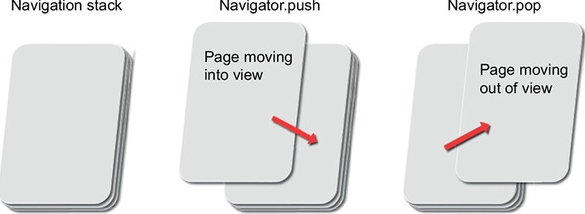
\includegraphics[scale=0.2]{../libs/navigation-stack}
				\end{figure}
			\end{column}
			\begin{column}{0.6\textwidth}
				\emph{Le singole pagine sono gestite come uno stack:}
				\begin{itemize}
					\item La pagina in cima allo stack è quella visibile
					\item Possiamo inserire una nuova pagina in uno stack con un \emph{push}
					\item Rimuovere la pagina corrente dallo stack e visualizzare quella sottostante con un \emph{pop}
					\item In alterntiva si può rimpiazzare la pagina corrente con un'altra con un \emph{pushReplacementNamed}
				\end{itemize}
			\end{column}
		\end{columns}
	\end{minipage}
\end{frame}

%% ---------------------------------------------------------------------------

\begin{frame}{Navigator}
	\emph{Oggetto Navigator}
	\begin{itemize}
		\item Possiamo recuperare l'oggetto \emph{Navigator} dal contesto come per il tema ed il media qury
		\item Attraverso questo oggetto possiamo poi effettuare le operazioni di push e pop
		\item In questo modo possiamo passare i parametri direttamente al widget
	\end{itemize}
	\centering
	\href{https://docs.flutter.dev/cookbook/navigation/navigation-basics}{\beamergotobutton{Documentazione}}
\end{frame}

%% ---------------------------------------------------------------------------

\begin{frame}{Passaggio di parametri}
	\emph{Possiamo passare i parametri in entrambe le direzioni:}
	\begin{itemize}
		\item Nel momento in cui si effettua \emph{push} di una nuova pagina
		\item Nel momento in cui si effettua il \emph{pop} di una pagina
	\end{itemize}
	\centering
	\href{https://docs.flutter.dev/cookbook/navigation/returning-data}{\beamergotobutton{Diamo una occhiata!}}
\end{frame}

%% ---------------------------------------------------------------------------

\section{Named Routes}
\begin{frame}{Named Routes}
	\emph{Organizzazione delle rotte:}
	\begin{itemize}
		\item Possiamo organizzare le nostre routes in modo più strutturato
		\item Per fare questo possiamo utilizzare le \emph{NamedRoutes}
		\item In questo caso è richiesto un po' di codice per il passaggio di parametri
	\end{itemize}
	\centering
	\href{https://docs.flutter.dev/cookbook/navigation/named-routes}{\beamergotobutton{Documentazione}}
\end{frame}

%% ---------------------------------------------------------------------------

\begin{frame}{Named Routes}
	\emph{Usare le named routes ci permette anche di avere più controllo sul cambio pagina:}
	\begin{itemize}
		\item Con \emph{onGenerateRoute} intercettiamo ogni pushNamed che non ha avuto esito tra le routes registrate e gestiamo la richiesta attraverso una funzione che restituisce una pagina
		\item Con \emph{onUnknownRoute} gestiamo le rotte sconosciute, dopo che onGenerateRoute non ha restituito alcuna vista
	\end{itemize}
	\centering
	\href{https://medium.com/flutter-community/flutter-navigation-cheatsheet-a-guide-to-named-routing-dc642702b98cs}{\beamergotobutton{Diamo una occhiata!}}
\end{frame}

%% ---------------------------------------------------------------------------


\section{Esercitazione}
\begin{frame}{Migliorare la precedente esercitazione}
	\begin{minipage}[0.2\textheight]{\textwidth}
		\begin{columns}[T]
			\begin{column}{0.4\textwidth}
				\begin{figure}[htpb]
					\centering
					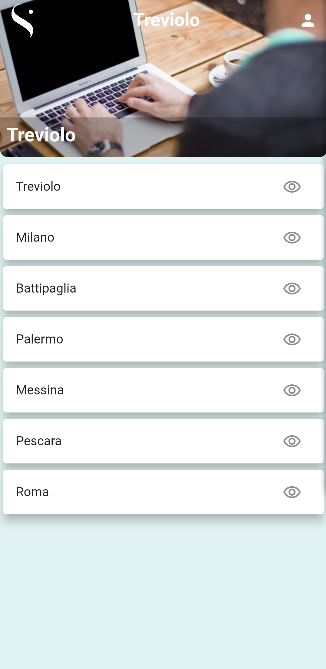
\includegraphics[width=2cm]{../libs/assignment-2-home}
				\end{figure}
			\end{column}
			\begin{column}{0.6\textwidth}
				\emph{Alcuni spunti:}
				\begin{itemize}
					\item Creare due nuove pagine: visualizzazione presenze di una sede e visualizzazione dati profilo;
					\item Alla visualizzazione delle presenze si accede mediante l'elemento in lista in home
					\item Alla pagina profilo si accede tramite l'icona del profilo in alto a destra nella AppBar in home formato portrait
					\item Fare in modo che al click in alto a sinistra su un'icona di home oppure il logo di SI2001, si ritorni alla home
					\item In pagina presenze, non dobbiamo mostrare il pulsante di \emph{back}
				\end{itemize}
			\end{column}
		\end{columns}
	\end{minipage}
\end{frame}


%% ---------------------------------------------------------------------------

% Reference frames
%%\begin{frame}[allowframebreaks]
%%    \frametitle{Riferimenti}
%%    \printbibliography
%%\end{frame}

%% ---------------------------------------------------------------------------
% Final frame
\section{Fine}
\begin{frame}{}
	\huge\emph{Grazie per l'attenzione!}
	\newline
	\vfill
	\hfill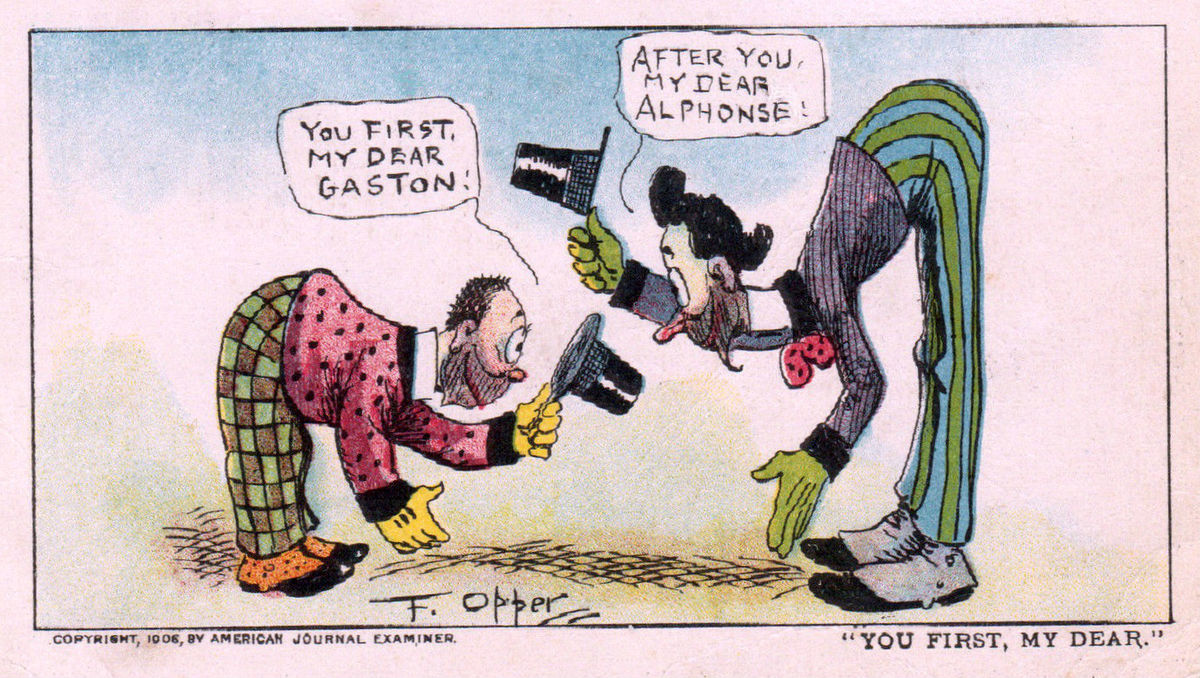
\includegraphics[width=6cm]{../libs/alphonse-gaston-regards}
\end{frame}

\end{document}